%%%%%%%%%%%%%%%%%%%%%%%%%%%%%%%%%%%%%%%%%%%%%%%%%%%%%%%%%%%%%%%%%%%%%%%%%%%%%%%%
%% LaTeX Simple LTU Slides Class Example File
%%
%% Created by: Roland Hostettler, April 4, 2011
%%
%% This example file shows you how to use the ltuslides.cls LaTeX class file to 
%% create simple presentations using the LTU profile, a clean background and
%% LaTeX.
%%%%%%%%%%%%%%%%%%%%%%%%%%%%%%%%%%%%%%%%%%%%%%%%%%%%%%%%%%%%%%%%%%%%%%%%%%%%%%%%

% Define the documentclass as 'ltusimple'
% =======================================
\documentclass{rhsleek}

% Load other packages, etc.
% =========================
\usepackage[utf8]{inputenc}
\usepackage{graphicx}
\usepackage[T1]{fontenc}

% PDF tweaks
% ==========
\usepackage[plainpages=false,pdfpagelabels]{hyperref}

% hyperref package settings
\hypersetup{
%	 bookmarks=true,                % show bookmarks bar?
%    unicode=false,                 % Non-Latin characters in bookmarks
%    pdftoolbar=true,               % Show toolbar?
%    pdfmenubar=true,               % Show menu?
%    pdffitwindow=false,            % Window fit to page when opened
%    pdfstartview={FitH},           % Fits the width of the page to the window
%    pdftitle={},                   % Title
%    pdfauthor={Roland Hostettler}, % Author
%    pdfsubject={},                 % Subject
%    pdfcreator={pdfTeX},           % Creator
%    pdfproducer={},                % Producer of the document
%    pdfkeywords={},                % List of keywords
%    pdfnewwindow=true,             % Open links in new windows
%	 pdfpagemode={FullScreen},      % Enable this for automatic full-screen view
    colorlinks=true,               % False: boxed links; true: colored links
    linkcolor=black,               % Color of internal links
    citecolor=black,               % Color of links to bibliography
    filecolor=black,               % Color of file links
    urlcolor=black,                % Color of external links
}

% Start the document
% ==================
\begin{document}


% Title slide
% ===========
% Note that we don't need to enclose this slide in a "slide"-environment
\title{\LaTeX~\texttt{ltuslides} Example}
\author{Roland Hostettler}
\affilation{Division of Systems and Interaction\\
Department of Computer Science, Electrical and Space Engineering\\
Luleå University of Technology}
\date{\today}
\maketitle


% A regular slide where you're completely free to design it
% =========================================================
\begin{slide}{Simple Bullet Lists}
	\begin{itemize}
		\item First item\\
		    {\small \dots with some small text below.}

		\item Second item\\
		    {\small \dots with some more text.}

		\item Falsches Üben von Xylophonmusik quält jeden größeren Zwerg.\\
		    {\small \dots it really does!}

		\item \dots\\
		    {\small \dots and so forth \dots}
	\end{itemize}
\end{slide}


% Another regular slide with some text and an image centered
% ==========================================================
\begin{slide}{Text \& Image}
	\begin{itemize}
		\item The picture below was taken from www.flickr.com/photos/-\_ra3yat\_bmw\_-/3144132890 (licensed as CC BY 2.0)
	\end{itemize}
	\vspace{0.5cm}
	\begin{center}
		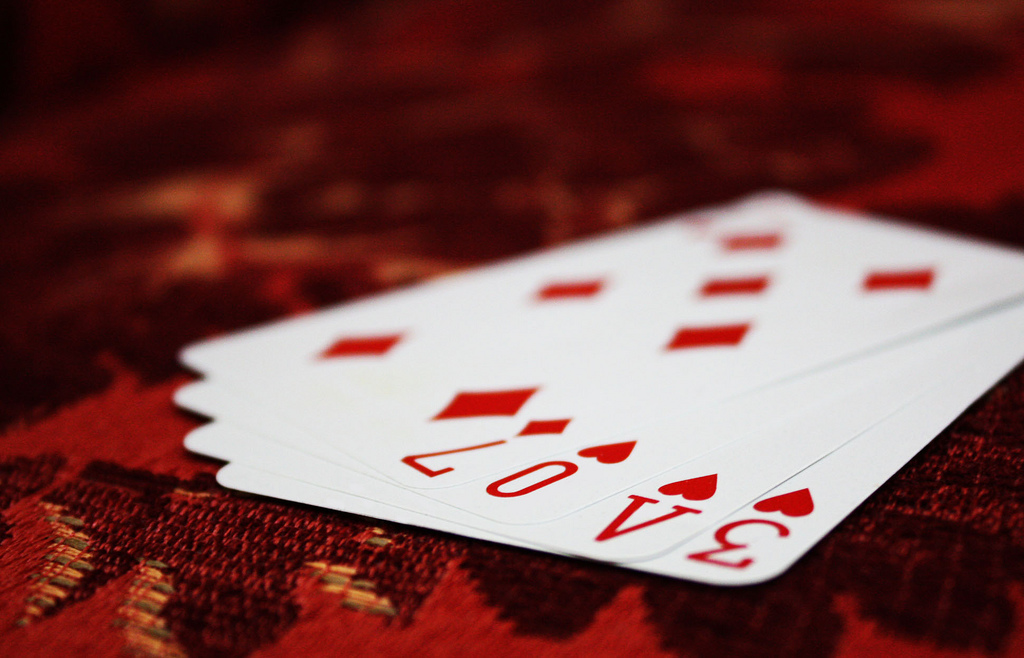
\includegraphics[width=0.4\textwidth]{template/example}
	\end{center}
\end{slide}


% A slide that has two columns
% ============================
% The first column...
\begin{slide}{Two Columns}
	\begin{column}
		\subsection{Column 1}
		\begin{itemize}
			\item You create slides with two columns using the environments \texttt{slide} and \texttt{column}
			\item Some text using \texttt{itemize} on the left and the right
			\item Note how the columns are nicely aligned at the top
		\end{itemize}
	\end{column}
	% ...and the second column. Note: Make sure there's no whitespace in between here!
	\begin{column}
		\subsection{Column 2}
		\begin{itemize}
			\item Note that the \texttt{column} environment doesn't take a parameter
			\item If you want to add column titles like on this slide, just use \texttt{subsection} above your \texttt{itemize}.
		\end{itemize}	
	\end{column}
\end{slide}

% A slide with two columns and an image on the right
% ==================================================
\begin{slide}{Two Columns, One Picture}
	\begin{column}
		\begin{itemize}
			\item Sometimes, you might want to have a picture besides text
			\item This slide shows an example for that
			\item It also uses \texttt{slide} and \texttt{column}
			\item Note that the image is centred horizontally in its column using the \texttt{center} environment
		\end{itemize}
	\end{column}
	\begin{column}
		\begin{center}
			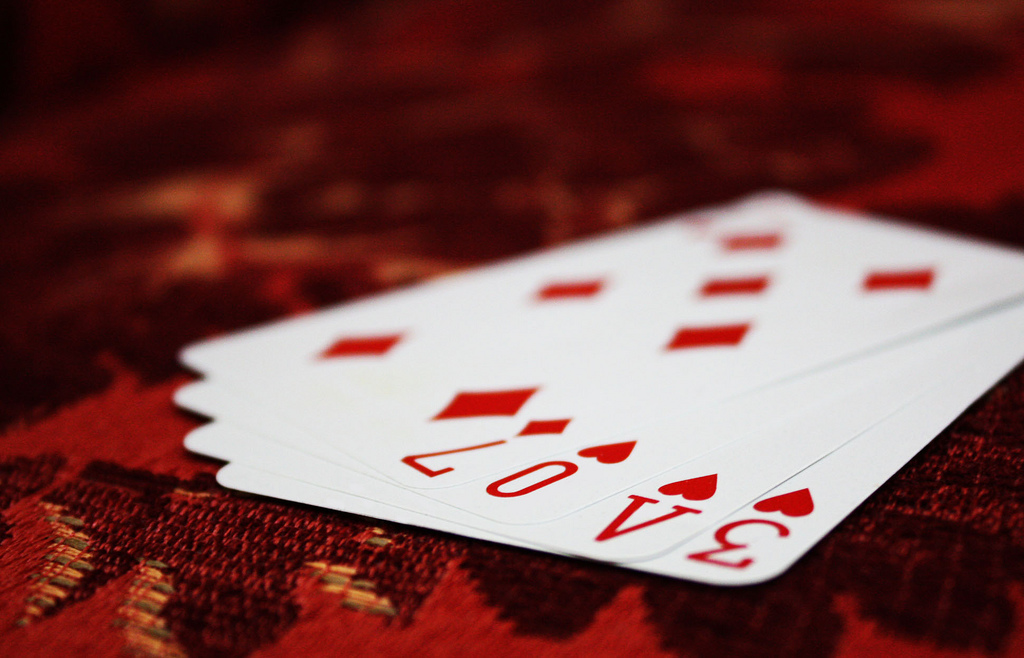
\includegraphics[width=0.8\textwidth]{template/example}
		\end{center}
	\end{column}
\end{slide}


% A slide with two columns on the top and an image at the bottom
% ==============================================================
\begin{slide}{Two Columns on Top, an Image at the Bottom}
	\begin{column}
		\begin{itemize}
			\item You can also place two columns besides each other on top (or at the bottom for that matter) and some content at the bottom, as done here
		\end{itemize}
	\end{column}
	\begin{column}
		\begin{itemize}
			\item Just always make sure that everything fits on one slide, otherwise it might get ugly
		\end{itemize}
	\end{column}
	\begin{center}
		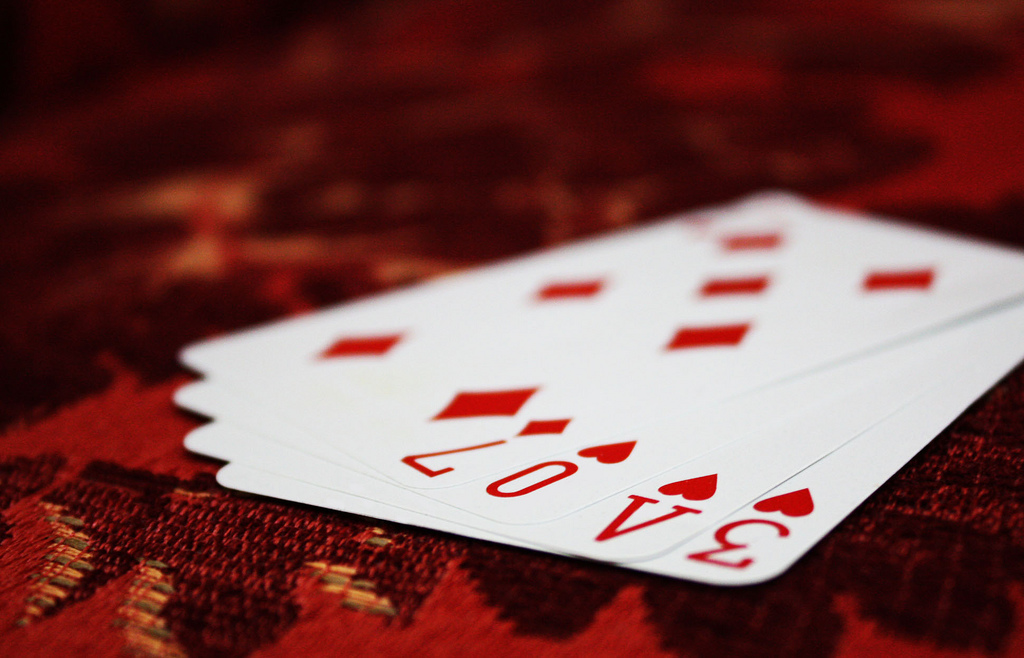
\includegraphics[width=0.4\textwidth]{template/example}
	\end{center}
\end{slide}


\end{document}

